\documentclass{article}
\usepackage[portrait, margin=1in]{geometry}
\usepackage{graphicx} 
\graphicspath{{/Users/danpost/consumer_sentiment/output/umich_figures/gaspx}}
\usepackage{amsmath}
\usepackage{hyperref}

\begin{document}

\section{University of Michigan Survey of Consumers Gas Expectations and Partisan Affiliation}

This memo summarizes the correlational relationship between observed gas prices and predicted gas prices among respondents of the University of Michigan's Surveys of Consumers Microdata. University of Michigan only began to reliably ask about respondents' political affiliation starting in late 2017.\footnote{The 1-year gas and 5-year gas price expectations are based on the questions 'GAS1' and 'GAS5' on the survey, asking respondents to predict how much gas prices will have changed within the next 1 and 5 years, respectively. \\  Information on respondents' partisan affiliation is taken from the question 'POLAFF'. \\ Information on the survey variables can be found \href{https://sda.umsurvey.org/sca/Doc/sca.htm}{here}. \\ All gas price data is taken from the Energy Information Administration (\href{https://www.eia.gov/dnav/pet/hist/LeafHandler.ashx?n=pet&s=emm_epm0_pte_nus_dpg&f=m}{EIA}).}

\subsection{Average Gas Price Expectations Over Time By Partisan Affiliation}

These plots are simple averages of gas price expectations by partisan affiliation collapsed on month-year. Independents, Republicans, and Democrats' gas price expectations were similar matching until around Joe Biden's election/inauguration (denoted by the two red vertical dashed lines), when Republicans' expectations spiked and, to a lesser extent, so did Independents'. During the Biden presidency, each of the three groups followed roughly similar trends, at different levels. \\

\centering 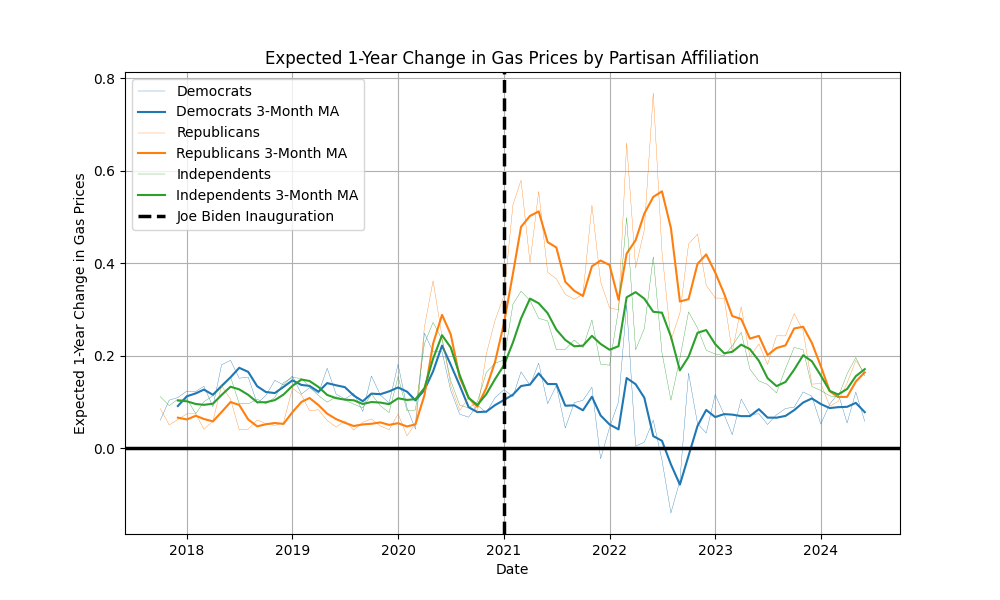
\includegraphics[width=4.5in]{gas1_party_comp.png} \\
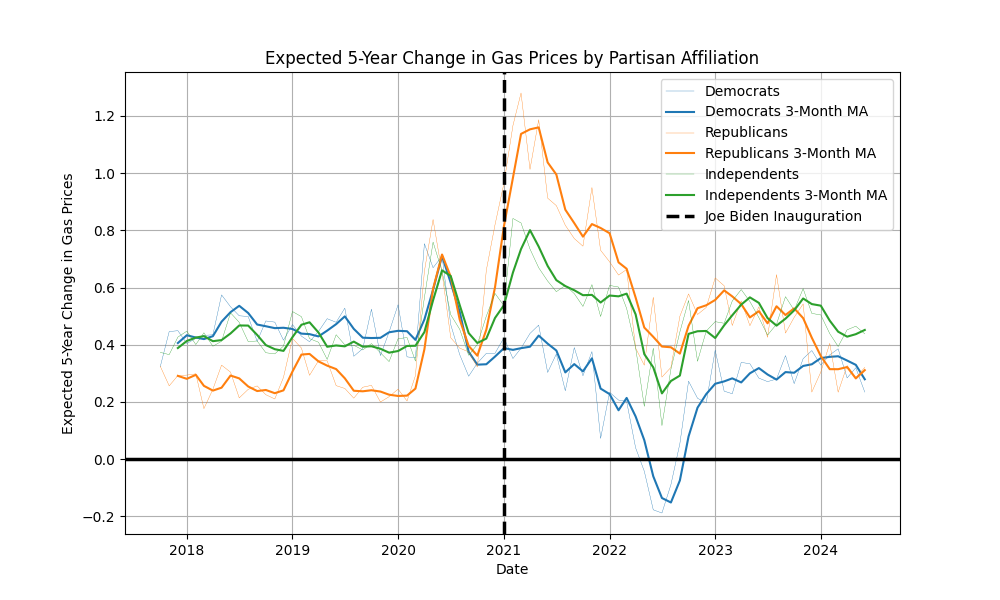
\includegraphics[width=4.5in]{gas5_party_comp.png}

\raggedright \subsection{Comparing Regressors} 
For context, here is a basic time-series comparing the regressors used in the various models above: \\
\vspace{0.1in}
\centering 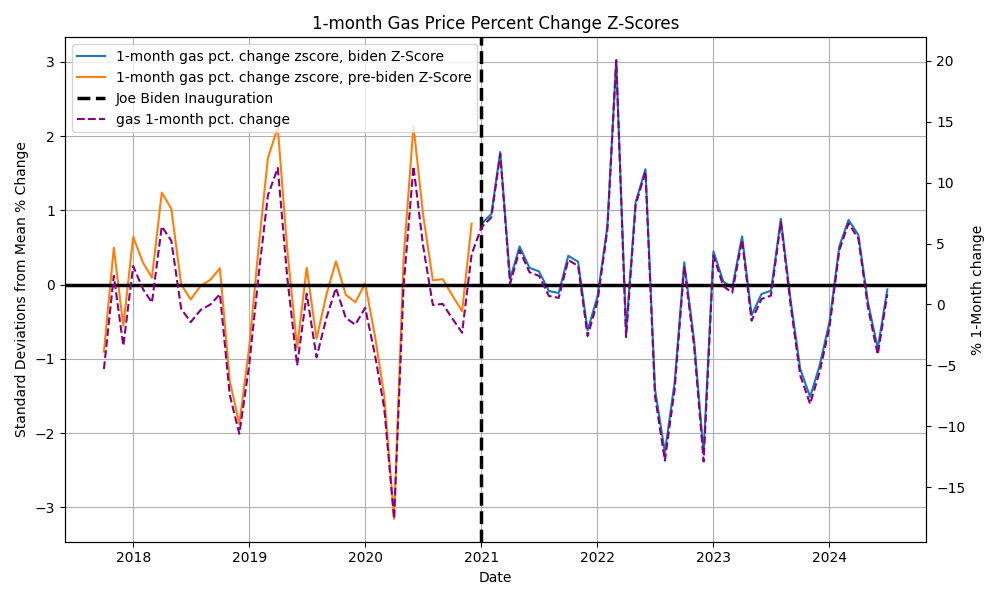
\includegraphics[width=4.5in]{1-month_gas_zscore_time_series.png} 
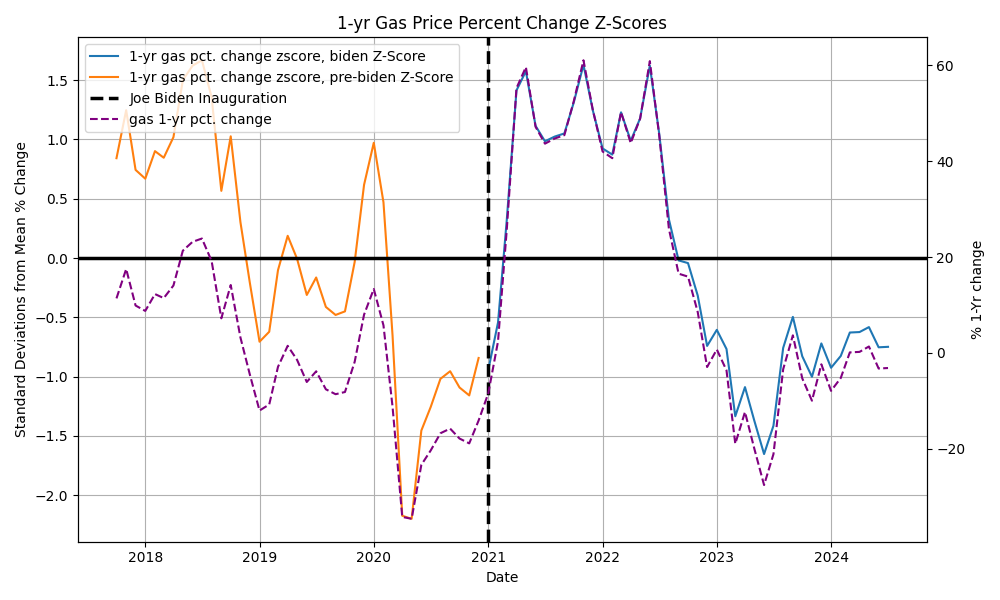
\includegraphics[width=4.5in]{1-yr_gas_zscore_time_series.png} 
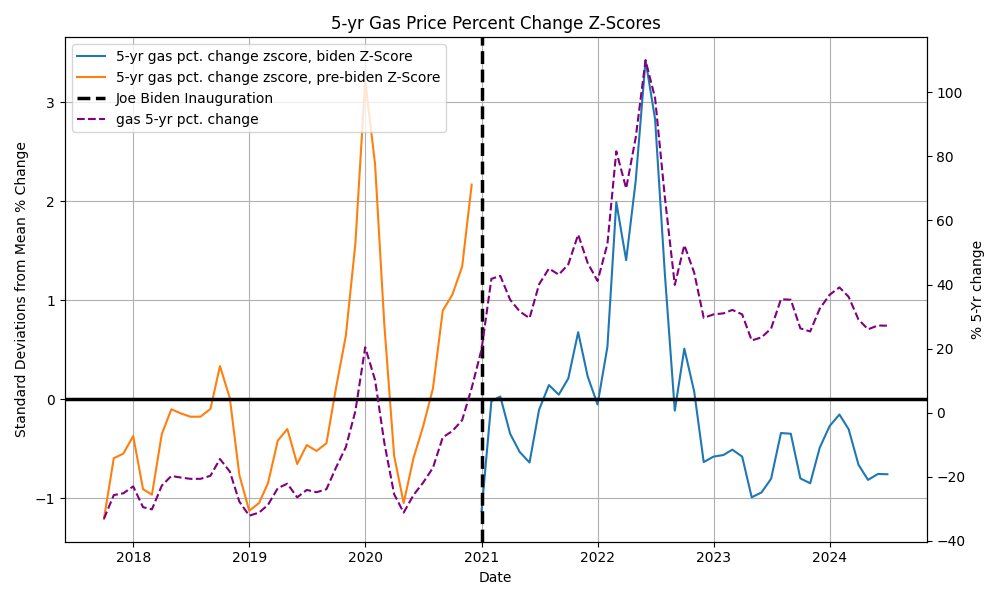
\includegraphics[width=4.5in]{5-yr_gas_zscore_time_series.png} 

\raggedright \subsection{Gas Price Monthly Difference Model}

\noindent For all of the following models, I run separate regressions for sub-samples organized around 1) partisan affiliation (democrats, republicans, and independents), 2) by whether Joe Biden is president or not (the Biden sub-sample begins January, 2021, and 3) for individuals' 1-year and 5-year gas expectations. Therefore, between models, \textbf{only the regressor changes}. In order to properly scale the observed gas price changes, I use the z-score of a monthly, yearly, or 5-year gas price change for 1) the Biden presidency, where there was greater variance in short-term gas price changes and 2) prior to the Biden presidency, where there was lesser variance in short-term gas price changes. 

The gas price monthly difference model is represented by this equation:
\begin{gather}
	 \text{GAS\_PX\_CHG\_EXP}_{h\text{, }p\text{, }t\text{, i}} = \alpha_0 + \beta_1 Z(\text{GAS\_PX\_CHG}_t) + \epsilon_{h\text{, }p\text{, }t\text{, i}}
\end{gather}
where $\Delta \text{GAS\_PX}_e\text{, horizon}$ is the individuals' expected price change in gasoline and $\Delta \text{GAS\_PX}$ is the change in nominal gas price level from the previous month. For both 1-year and 5-year gas price expectations, I use the month-by-month change in gas prices as the independent variable. \\
\vspace{0.1in}
As expected, respondents' gas price expectations during the Biden presidency, when there was significant volatility in gas prices, are significantly positively correlated with month-to-month changes in gas price expectations. While Democrats' and Independents' exhibit similar correlational strengths, Republicans appear significantly more sensitive to gas price changes during the Biden presidency than either Democrats or Independents, although this pattern also appears to hold for when Trump was president. \\
\vspace{0.1in}
\centering 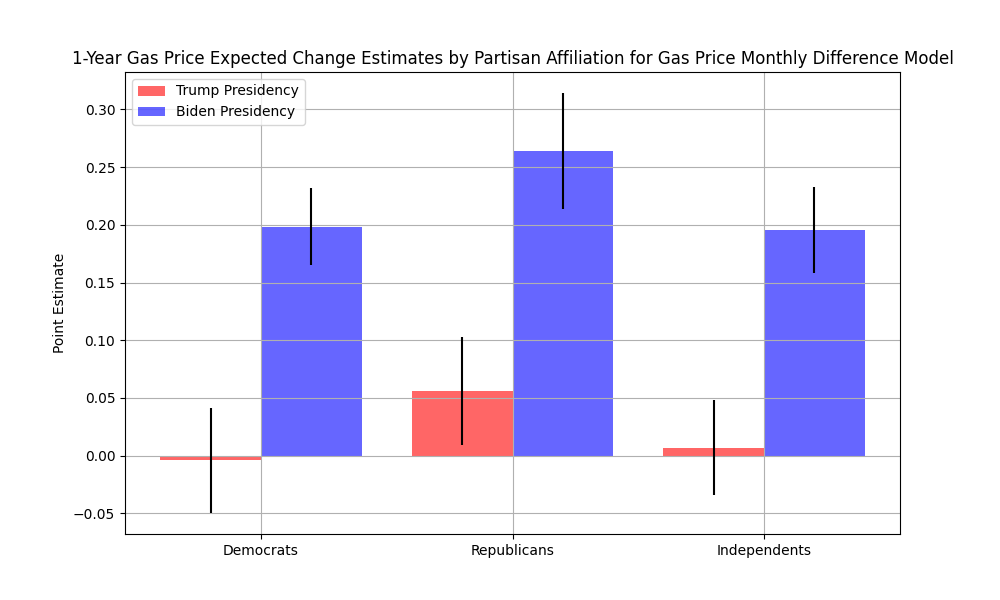
\includegraphics[width=4.5in]{model_month_chg_gas1_party_comp.png} \\
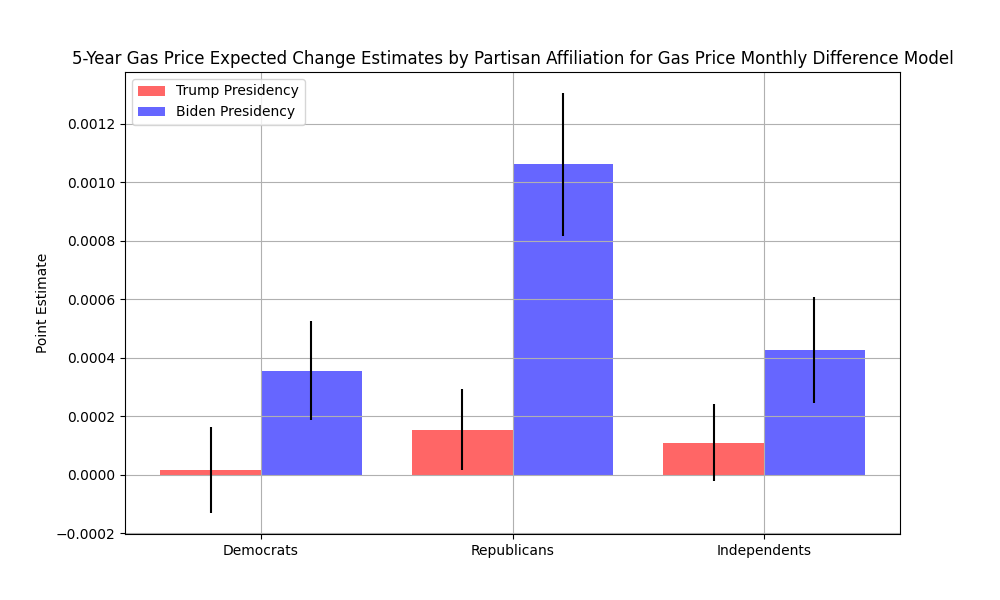
\includegraphics[width=4.5in]{model_month_chg_gas5_party_comp.png} 

\raggedright \subsection{Gas Price Precise Difference Model}
The gas price precise difference model is represented by this equation:
\begin{gather}
	 \text{GAS\_PX\_CHG\_EXP}_{h\text{, }p\text{, }t\text{, i}} = \alpha_0 + \beta_1 \text{GAS\_PX\_CHG}_{t\text{, }h} + \epsilon_{h\text{, }p\text{, }t\text{, i}}
\end{gather}
where $\Delta \text{GAS\_PX}_{\text{horizon}}$ is the observed historical gas price change matched to the horizon of gas price expectations. Thus, for 1-year gas price expectations, I find the historical 12-month gas price level change and for 5-year expectations, I find the historical 5-year gas price level change. Therefore, if individuals' predicted price changes perfectly matched what happened historically, $\beta_1$ would be 1. \\
\vspace{0.1in}
These findings are more drastic: Democrats exhibit largely no responsiveness to one-year gas price changes for either the Biden or Trump Presidency, while Republicans flip the sign of their sensitivity from the Trump to Biden presidency and Independents appear to be somewhere in between Republicans and Democrats in the strength of their correlation. For 5-year gas price changes, the results are complicated by the sign of 5-year gas price changes: during the Trump presidency, 5-year historical gas price changes were almost entirely negative. It's not clear why the coefficients for the Biden Presidency 5-year expectations are so significantly negative--this requires further data analysis. \\
\vspace{0.1in}
\centering 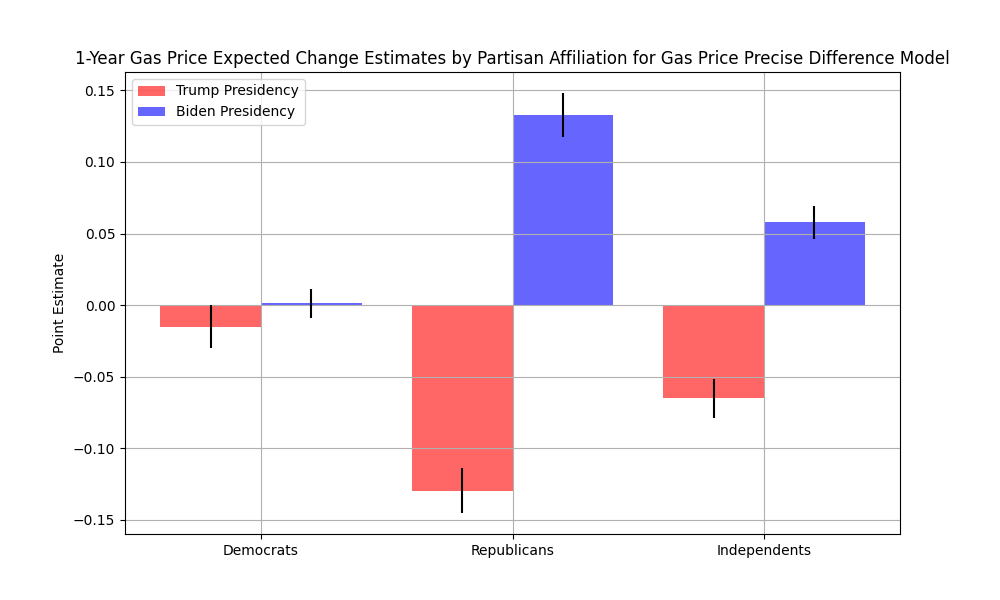
\includegraphics[width=4.5in]{model_precise_chg_gas1_party_comp.png} \\
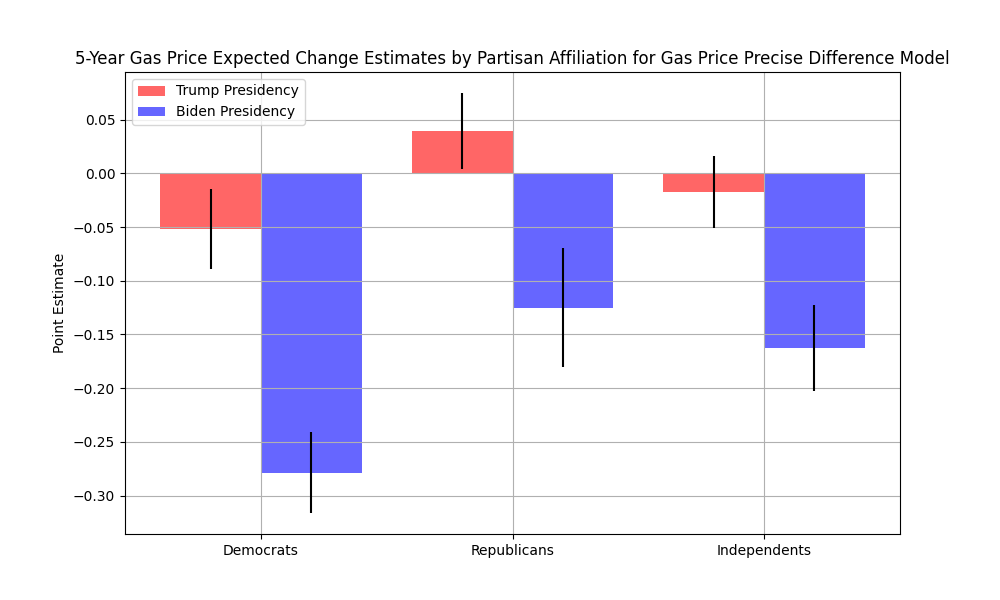
\includegraphics[width=4.5in]{model_precise_chg_gas5_party_comp.png} 

\raggedright \subsection{Gas Price Levels Model}
The gas price levels model is represented by this equation:
\begin{gather}
	 \text{GAS\_PX\_CHG\_EXP}_{h\text{, }p\text{, }t\text{, i}} = \alpha_0 + \beta_1 \text{GAS\_PX}_t + \epsilon_{h\text{, }p\text{, }t\text{, i}}
\end{gather}
where GAS\_PX is the level gas price the month that an individual is predicting the future gas prices.\\
\vspace{0.1in}
The gas price levels model tells a similar story to the gas precise difference model -- Republicans flip the correlational direction between their expected change and observed gas prices when Joe Biden became President. \\
\vspace{0.1in}
\centering 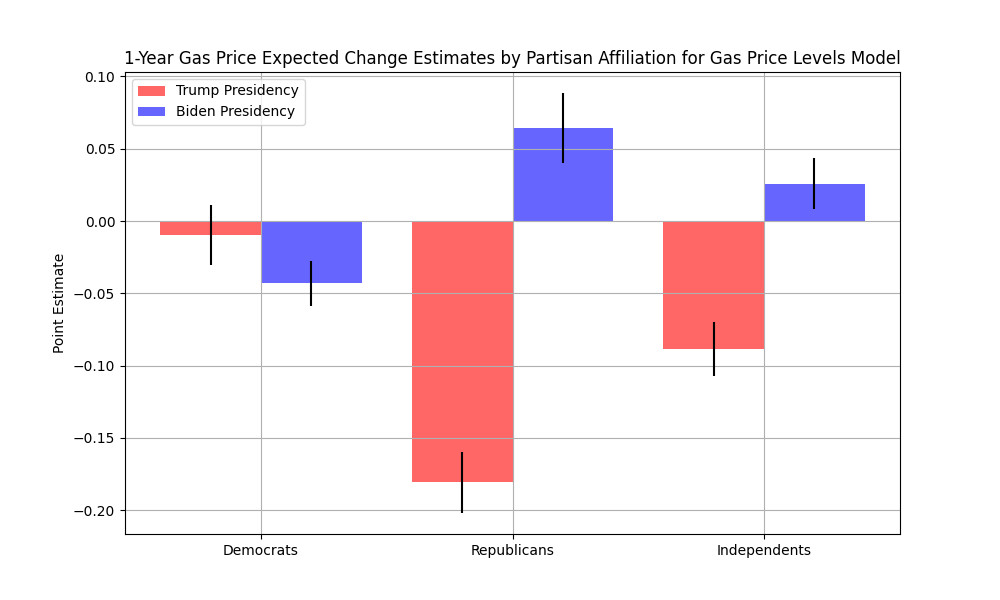
\includegraphics[width=4.5in]{model_level_gas1_party_comp.png} \\
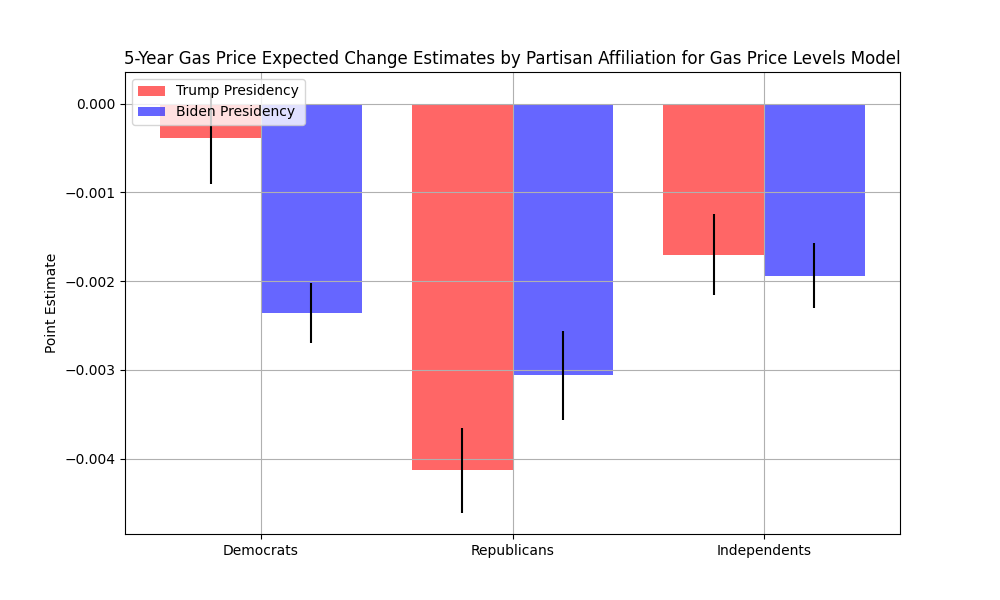
\includegraphics[width=4.5in]{model_level_gas5_party_comp.png} 

\end{document}